\patternFour

\subsection*{Context}

    Time series are widely used in science and engineering. Examples are the results of experiments, laboratory analyses or simulation results.
Such data is usually represented as a sequence of tuples (time | value). 
To analyze and interpret such results, they are displayed visually as graphs.
    
\subsection*{Problem}

\begin{itshape}

Graphical representations of time series  are not accessible for \ac{bvi} students and people in general. A sequential output of the data on Braille lines or by means of text-to-speech is not well suited to represent and convey the time based aspect of the data.   

\end{itshape}

\subsection*{Solution}


\begin{sol}

Provide sonifications of time series.
\end{sol}

Sonification is the use of non-speech audio to convey information.
For a time series  $x(t)$, data points can be mapped to sound parameters:
amplitude, rate of change, loudness or stereo position etc. 
\ac{bvi} students can listen as time unfolds, effectively hearing the trend.

Advanced sonification techniques comprise spatial audio (3D audio, auralization), where time or value is represented by left–right panning for added dimensionality.



\subsection*{Examples}

Highcharts\footnote{\url{https://www.highcharts.com/}}, in collaboration with the Sonification Lab at the Georgia Institute of Technology, has developed a free tool that enables the exploration of time series as charts and their sonification, employing sound as a medium for data visualization.

The charging of a capacitor is covered in \ac{stem}courses  for several reasons: it illustrates central concepts important in many disciplines, such as the creation of differential equations or the modeling and simulation of technical systems.

Fig.~\ref{fig:rc} shows a typical circuit for charging a capacitor via a resistor. The time constant $\tau$ is calculated from the product of the capacitance $C$ and the resistance value $R$: $\tau = R * C$.
The charging curve is described by the following formula: 


\[
U(t) = U_0 * (1- e^{-{ \frac{t}{\tau}}})
\]



\newpage
Listing \ref{lst:rc} shows the first 20 entries of a time series of charging a capacitor via a resistor($\delta t = 0.1$, $\tau = 2$).


\begin{lstlisting}[label=lst:rc, caption = time series of charging a capacitor]
t,U
0,0
0.1,0.48770575499286
0.2,0.951625819640405
0.3,1.39292023574942
0.4,1.81269246922018
0.5,2.21199216928595
0.6,2.59181779318282
0.7,2.95311910281287
0.8,3.29679953964361
0.9,3.62371848378227
1,3.93469340287367
1.1,4.23050189619513
1.2,4.51188363905974
1.3,4.77954223238984
1.4,5.03414696208591
1.5,5.27633447258985
1.6,5.50671035882778
1.7,5.72585068051273
1.8,5.93430340259401
\end{lstlisting}

This time series was imported and Highcharts generated the chart shown in Fig.~\ref{fig:sonification}. On top of the page, there are the buttons for playing the sound: Play, Stop and Loop.  

\begin{figure}
    \centering
    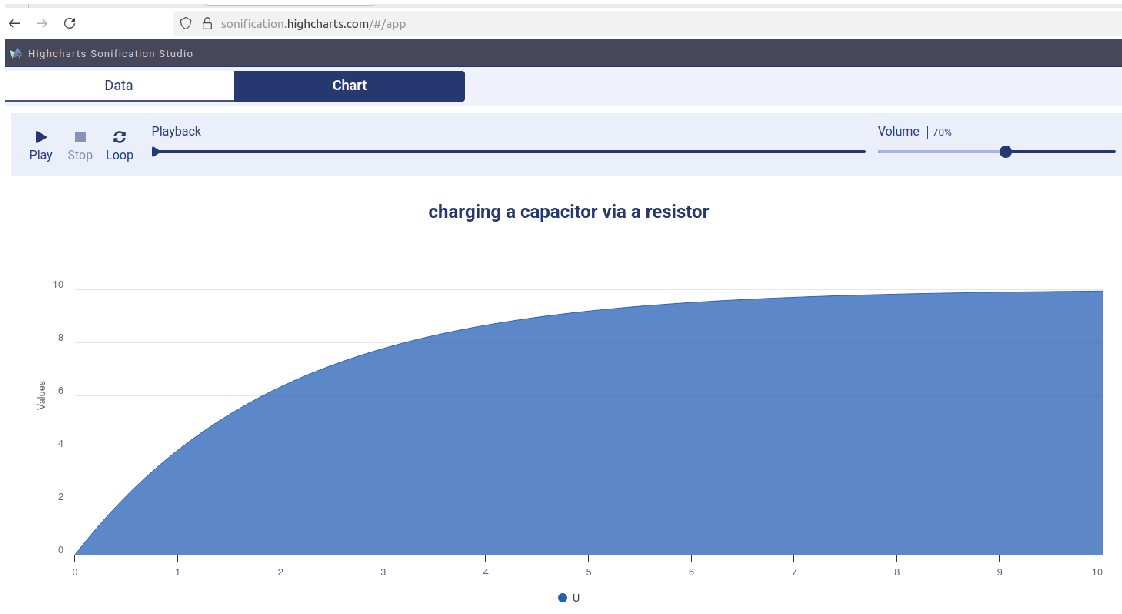
\includegraphics[width=\linewidth]{img/sonification.pdf}
    \caption{Screenshot from the sonification web site}
    \label{fig:sonification}
\end{figure}
 
\subsection*{Consequences}

% Benefits
\renewcommand{\labelenumi}{$+$}
\begin{enumerate}
\item Time series usually contain the temporal progression of signals; sonification allows the dimension of time to be experienced intuitively.

\item Some tools allow the playback speed to be adjusted or zoomed in on specific points in time.

\item Web-based solutions are easy to use for sonification and are usually easily accessible.

\end{enumerate}

% Liabilities
\renewcommand{\labelenumi}{$-$}
\begin{enumerate}
\item Understanding and correctly interpreting audible time series requires experience and training, among other things.

\item Devices for spatial audio reproduction are more expensive than normal headphones.

\item Sonification software usually needs to be installed, and training in the use of the software is necessary. 
\end{enumerate}
 
 
\subsection*{Related Work}

In \cite{potluri2022psst} Physical-computing Streaming Sensor data Toolkit (PSST) is introduced. This  toolkit enables \ac{bvi}  developers to create accessible representations of real-time sensor data. PSST allows users to filter, highlight, and transform time series of raw or computed sensor values into different output formats including tonal sonification, non-speech audio, speech, and SVG files for tactile displays. 

in \cite{casado2021} SonoUno is presented. It is a sonification software for astronomical data presented on a table (txt or csv files). Goal of the project is enabling accessibility to scientific data, from the Earth or with instruments on board of satellites. Such data is available in databases
such as Simbad, NASA, ESA, among others.

The study presented in \cite{Last2015} tested the hypothesis that musical sonification can serve as an effective alternative to visualizing time-series data when visual representation is unavailable or not accessible especially for \ac{bvi} people. The authors developed a time-series sonification method that can translate both uni-variate and multi-variate time series into a musical format.

In \cite{damsa2024}  a study examining the educational outcomes of \ac{bvi} children aged 0 to 8  learning  sonification concepts is presented. 
\ac{bvi} children  face significant barriers to participating in Science, Technology, Engineering, and Mathematics (STEM) education and careers, which have traditionally depended on visually based information. The authors had developed  an app „Sonoplanet“ for the sonification in an  educational context.
